\subsection{Implementation}

The entire system will be implemented exploiting a \textbf{bottom-up} approach. This approach is chosen for both the server side and the client side. The server side will be the first to be implemented and tested. A bottom-up implementation is incremental and gives the possibility to test whenever possible every small software unit regardless of the others facilitating bug tracking.\\
\newline
The first step can be implementing the DataManager which will be communicating with the DBMSService (MySQL) thanks to JDBC. This will guarantee to others components depending on the DataManager's interfaces to access to persistent objects mapped to the relational database.\\
\newline
After that we will implement the AuthManager component which depends only on the DataManager.\\
The next step consists in implementing the TicketManager.\\
MapsServiceServerAdapter will be implemented and tested before the BuildingManager as the latter depends on it.\\
\newline
Finally, for the server side, the dispatcher will be implemented.\\
\newline
The order in which we will implement our components in the application server is:

\begin{enumerate}[label=\arabic*]
 \item DataManager
 \item AuthManager
 \item TicketManager
 \item MapsServiceServerAdapter
 \item BuildingManager
 \item Dispatcher
\end{enumerate}

In parallel we will implement the MapsServiceMobileAdapter and the MobileApplication components.\\
\newline
DBMSService is not implemented as it is the DBMS software and neither is GoogleMapsService as it is an external service component.\\
\newpage

\subsection{Integration and Test Plan}

As stated previously we will use a bottom-up approach.\\
The following diagrams illustrates in each step how we will combine each component and which utility components will be used to test them.\\
\newline
\textbf{Server side}\\
\textbf{Step 1}:
The DataManager is tested with a Driver class that uses its interfaces.\\
\textbf{Step 2}:
After that it's the turn of AuthManager as it depends only on the DataManager already tested.\\
\textbf{Step 3}:
When integrating TicketManager we need a Stub Component in order to simulate the BuildingManager's WaitingTimeInt interface.\\
\textbf{Step 4}:
The MapsServiceServerAdapter, on which the BuildingManager will depend, is tested separately with the GoogleMapsService and a driver Class to simulate the calls to its offered methods.\\
\textbf{Step 5}:
Now that MapsServiceServerAdapter is implemented and tested we can integrate the BuildingManager and remove the stub class. This step is crucial as it handles most of the business logic's implementation. The Stub class is replaced with the BuildingManager component.\\
\textbf{Step 6}: Finally the Dispatcher can be implemented, integrated and tested with the rest of the server side system.\\
\newline
\textbf{Client Side}\\
\textbf{Step 7}: The MapsServiceMobileAdapter is implemented and tested with the GoogleMapsService and a Driver class to simulate the calls to its methods.\\
\textbf{Step 8}:
Final integration Step. MobileApplication and WebApplication are integrated into the whole system.
 
  \begin{figure}[H]
 \centering
 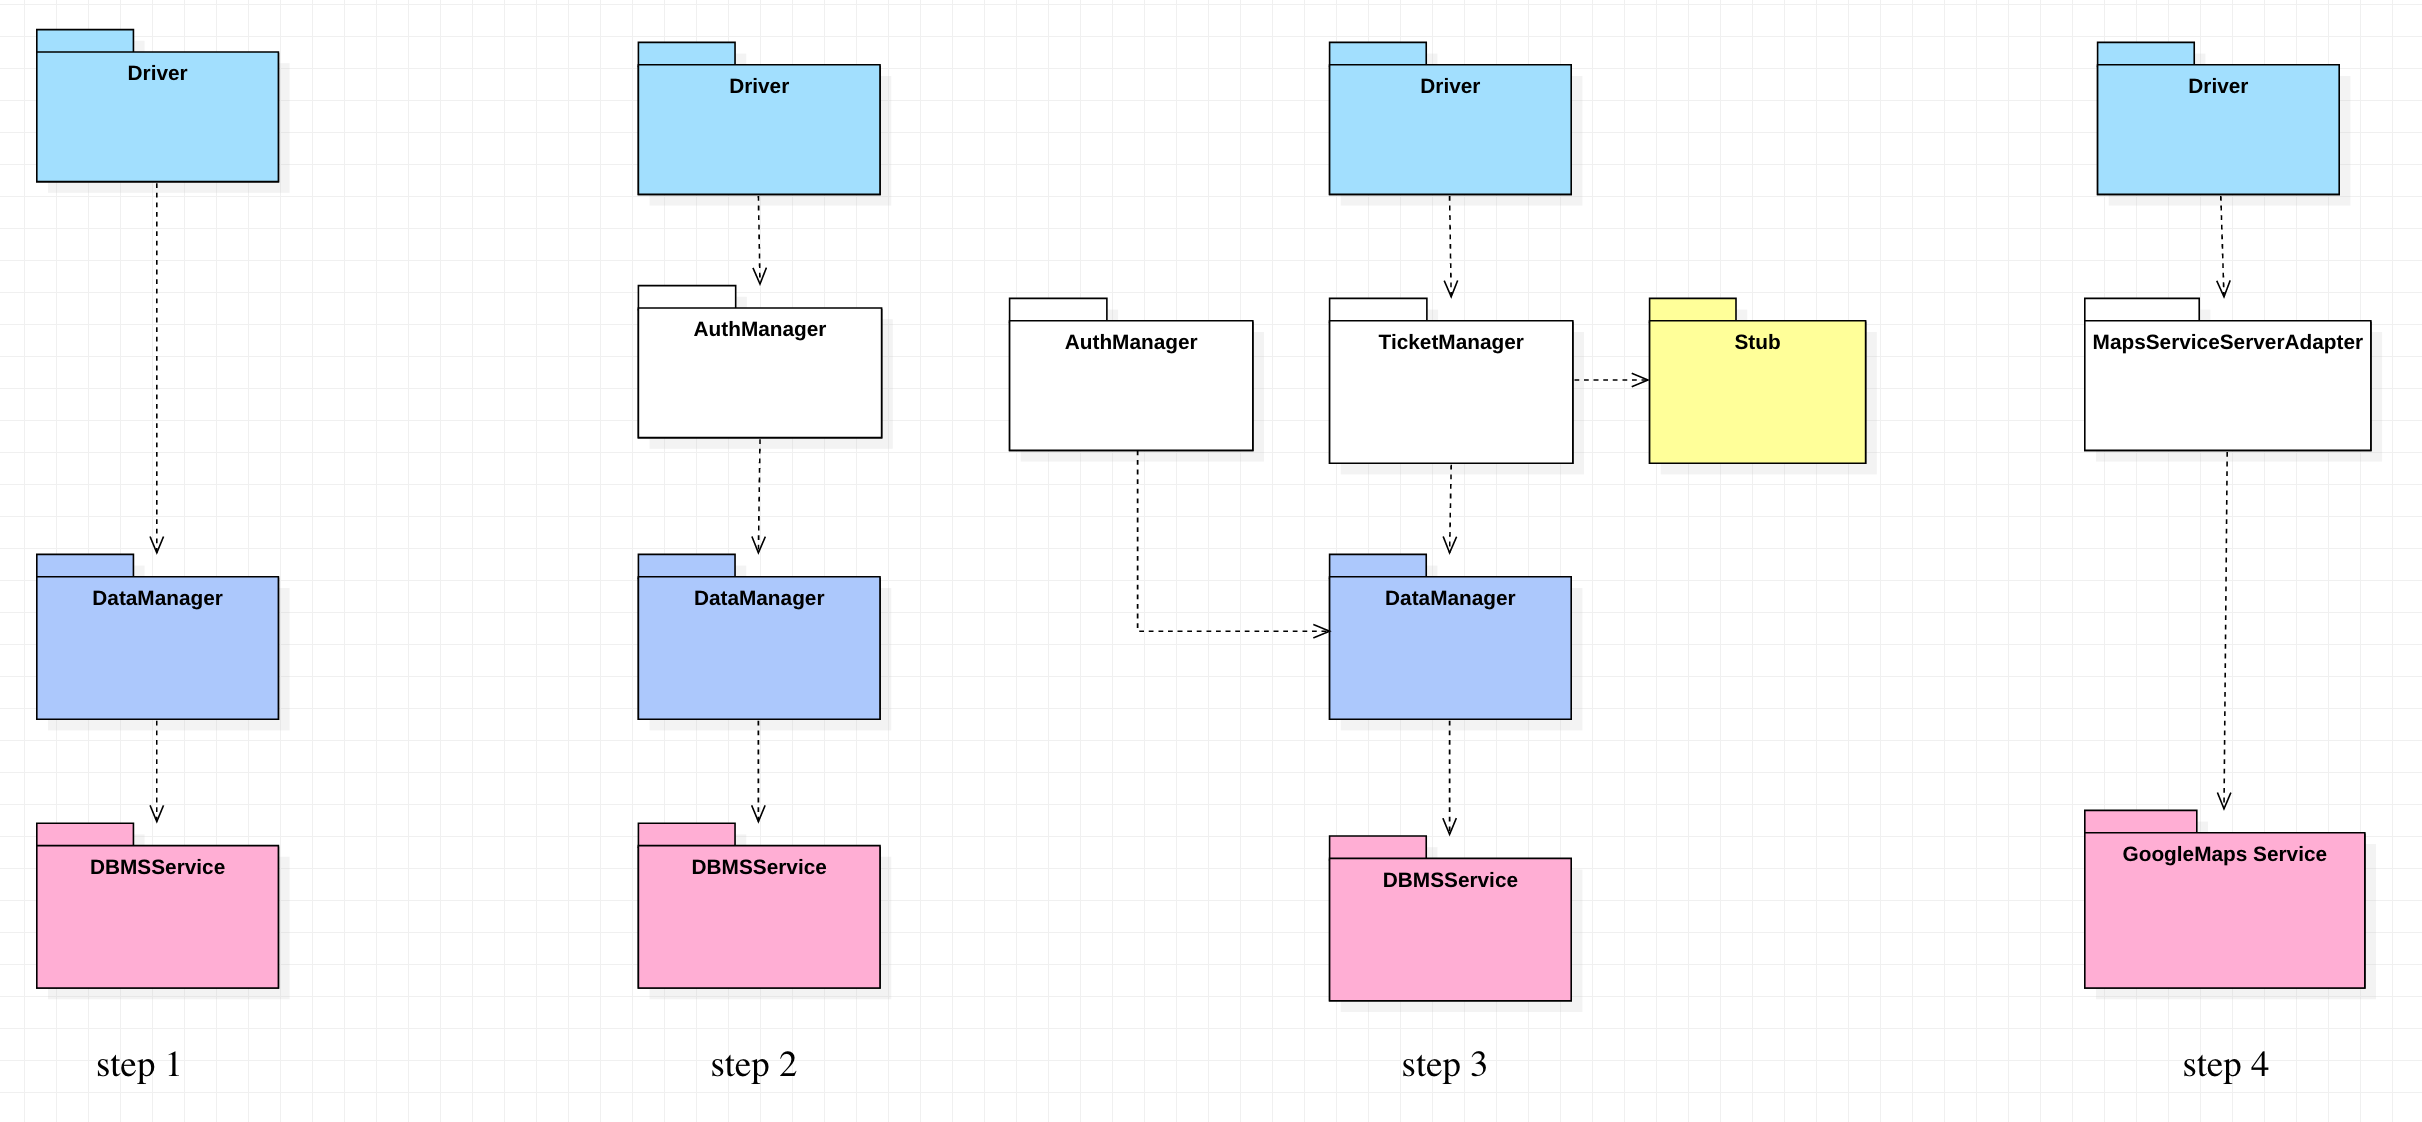
\includegraphics[width=\textwidth]{Diagrams/Integration1}
 \end{figure}
 
 \newpage
 
  \begin{figure}[H]
 \centering
 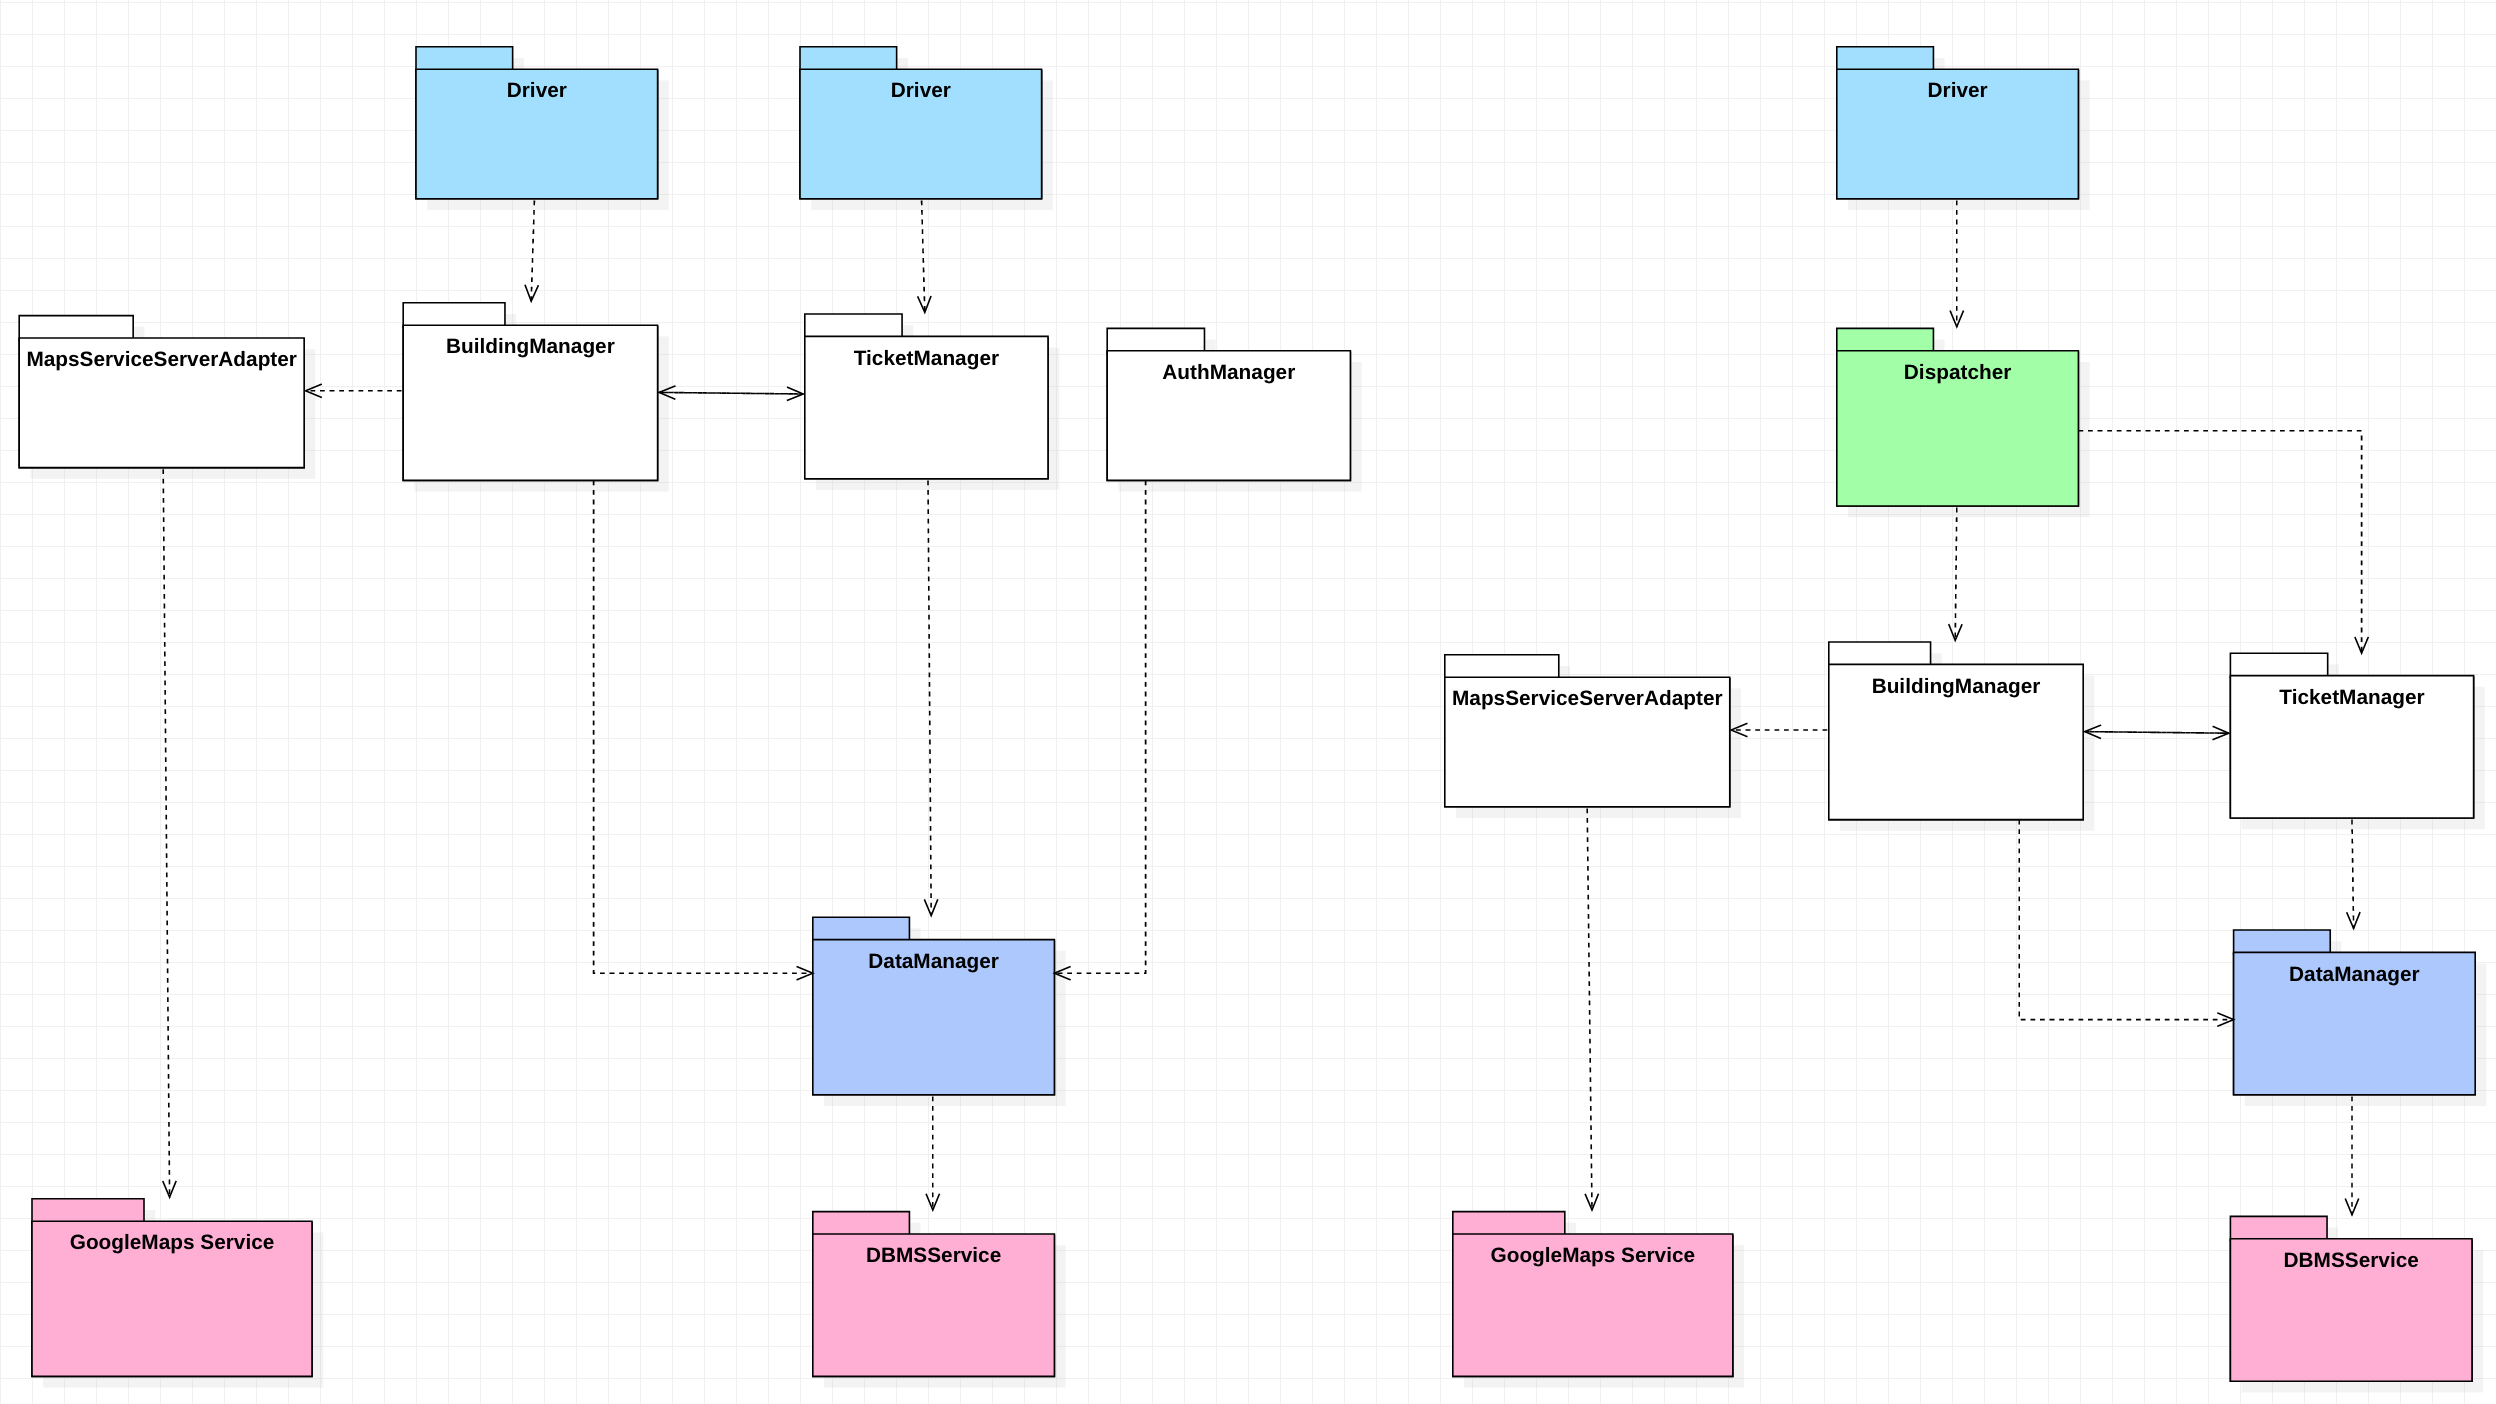
\includegraphics[width=\textwidth]{Diagrams/Integration2}
 \end{figure}
 
   \begin{figure}[H]
 \centering
 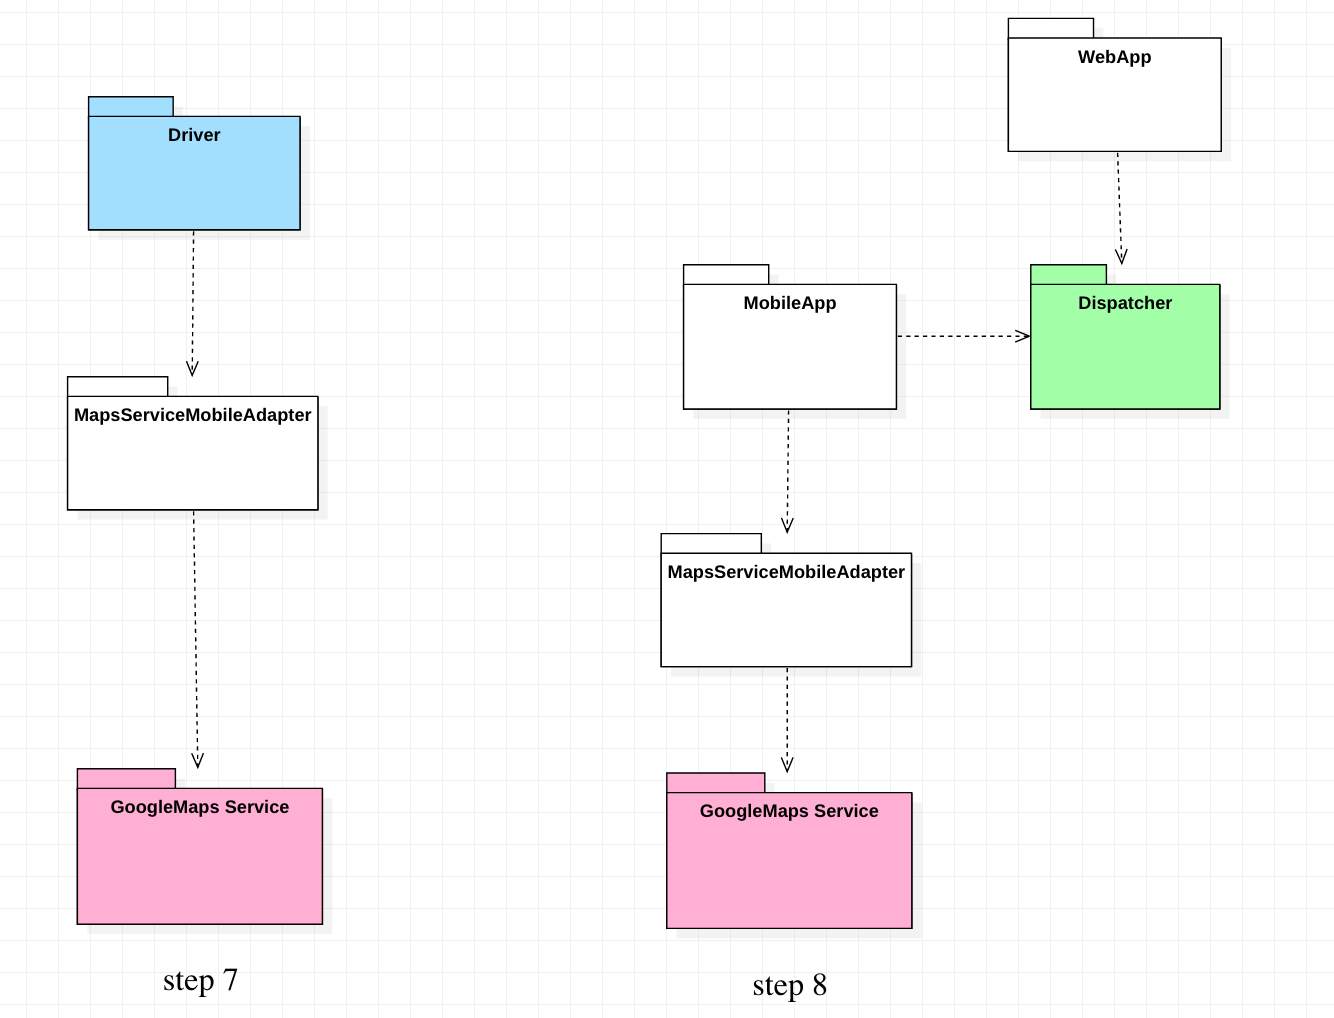
\includegraphics[width=\textwidth]{Diagrams/Integration3}
 \end{figure}
